%% \documentclass{report}
%% 
%% \usepackage{fancyhdr}
\usepackage{fourier-orns}
\usepackage{hyperref}%% To refrence links / jumps
\usepackage{chngcntr} %% For some extra counters numberings
\usepackage[a4paper, right = 0.5in, left = 0.5in,top = 1in , bottom = 1in]{geometry}
\usepackage{etoolbox} %% Provides like a language for advanced customization
\usepackage{datetime} %% For dates of course
\usepackage{lastpage} %% provides pages numbers
\usepackage[sc]{titlesec} %% modify titles
\usepackage{enumerate}
\usepackage{cancel}
\usepackage{tikzsymbols}
\usepackage[dvipsnames]{xcolor}
\usepackage{import}
\usepackage{pdfpages} %% include other pdfs
\usepackage{transparent} %% Transparency
\usepackage{xcolor}  %% Colors
\usepackage[many]{tcolorbox}
\usepackage[framemethod=TikZ]{mdframed}
\usepackage{amsmath,amsfonts,amsthm,amssymb,mathtools}
\usepackage{tikz}
\usepackage{bookmark}
\usepackage{graphicx}
\usepackage{mathpazo}

\usepackage{fontawesome5}

\linespread{1.5}


\titleformat{\chapter}[display]   
{\fontfamily{ppl}\selectfont\huge\color{YellowOrange!80!orange}} % Font style and size 
{\raggedleft\color{purple}\fontsize{70}{0pt}\selectfont\thechapter}   
{-1.5cm}    			                          % Space between the chapter number and title
{
	\begin{tikzpicture}[overlay]
		\node[anchor = west,yshift = 0.2cm,xshift = -1cm] {\fontsize{90}{20} $\int_{}^{} $};
		\node[yshift = 4cm, xshift = 17cm]   {\includegraphics[width = 4cm]{preview0}};
	\end{tikzpicture}
\hspace{1cm}\Huge\raggedright\MakeUppercase}

\titleformat{\section}[block]
{
\fontfamily{ppl}\selectfont\huge\color{YellowOrange!80!orange}
}
{
\color{purple}\fontsize{20}{0pt}\selectfont\thesection 
}
{0cm}
{
	\begin{tikzpicture}[overlay]
		\node[anchor = west,yshift = 0.2cm,xshift = -0.4cm, circle = 1pt] {};
	\end{tikzpicture}
}

\titlespacing*{\section}{0pt}{0.7cm}{1.5cm}


\newcommand{\divider}
{
	\begin{center}
	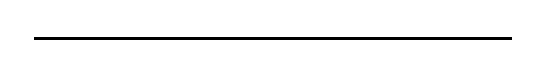
\begin{tikzpicture}
		\draw[thick, black] (0.25*\textwidth, 0) -- (0.75*\textwidth, 0);
		\node[rotate = 360 - 90, xshift = -0.6pt, yshift = 1pt] at (0.25*\textwidth,0){\decotwo};
		\node[rotate = 90, xshift = -0.6pt, yshift = 1pt] at (0.75*\textwidth,0){\decotwo};
	\end{tikzpicture}
	\end{center}
}

\pagestyle{fancy}

\newcommand{\lecday}[1][]
{
    \def\datee{#1}
    \fancyhead[L]{\datee}
}



\newcommand{\signature}
{
	\begin{tikzpicture}[remember picture,overlay]
		\node[fill = YellowOrange!20!white] at ([yshift = 1cm, xshift = -3cm]current page.south east) {\fontsize{10pt}{0pt}{\itshape Kara.$\mathcal{A}$}};
	\end{tikzpicture}
}

\AddToHook{shipout/background}{
  \begin{tikzpicture}[remember picture, overlay]
	  \node[] at ([yshift = 1.5cm,xshift = \textwidth /2 + 0.9cm]current page.south west) {\includegraphics[width = 0.5cm]{preview3}};
	  \node[] at ([yshift = 1.5cm,xshift = - \textwidth /2 - 0.9cm]current page.south east) {\includegraphics[width = 0.5cm]{preview4}};
  \end{tikzpicture}
}



\newtcolorbox[auto counter, number within = section]{remark}[1][]
{
       		title = Remark #1,
		enhanced,
		boxrule = 0pt,
		colback = white,
		breakable,
		arc = 4pt,
		colbacktitle = cyan,
		colback = cyan!5!white,
		segmentation style =
		{
			solid,cyan,thick,
		},
		attach boxed title to top left =
		{
			xshift = 0cm,
		},
		boxed title style =
		{
			boxrule = 0pt,
			sharp corners,
			drop fuzzy shadow = {cyan},
		},
		drop fuzzy shadow = {cyan!80!black},
}

\newtcolorbox[auto counter, number within = section]{theorem}[1][]
{                                      
		title = Theorem \thetcbcounter : #1,
		enhanced, 
		boxrule = 0pt,
		colback = white,
		breakable,
		arc = 4pt,
		colbacktitle = purple,
		colback = purple!5!white,
		segmentation style = 
		{
			solid, purple,thick,
		},
		attach boxed title to top left = 
		{
			xshift = 0cm, 
		},
		boxed title style = 
		{
			boxrule = 0pt,
			sharp corners,
			drop fuzzy shadow = {purple},
		},
		drop fuzzy shadow = {purple!80!black},
}

\newtcolorbox[auto counter, number within = section]{definition}[1][]
{                                      
		title = Definition \thetcbcounter : #1,
		enhanced, 
		boxrule = 0pt,
		colback = white,
		arc = 4pt,
		breakable,
		colbacktitle = YellowOrange!80!black,
		segmentation style = 
		{
			solid, YellowOrange,thick,
		},
		attach boxed title to top left = 
		{
			xshift = 0cm, 
		},
		colback = YellowOrange!5!white,
		boxed title style = 
		{
			boxrule = 0pt,
			sharp corners,
			drop fuzzy shadow = {YellowOrange!80!orange},
		},
		drop fuzzy shadow = {YellowOrange!80!black},
}

\newtcolorbox[auto counter, number within = section]{corollary}[1][]
{                                      
		title = corollary \thetcbcounter : #1,
		enhanced, 
		boxrule = 0pt,
		colback = white,
		arc = 4pt,
		breakable,
		colbacktitle = YellowOrange!80!black,
		segmentation style = 
		{
			solid, YellowOrange,thick,
		},
		attach boxed title to top left = 
		{
			xshift = 0cm, 
		},
		colback = YellowOrange!5!white,
		boxed title style = 
		{
			boxrule = 0pt,
			sharp corners,
			drop fuzzy shadow = {YellowOrange!80!orange},
		},
		drop fuzzy shadow = {YellowOrange!80!black},
}


\newtcolorbox{example}[1][]
{                                      
		title = Example,
		enhanced, 
		boxrule = 0pt,
		colback = white,
		arc = 4pt,
		segmentation style = 
		{
			solid, SpringGreen,thick,
		},
		breakable,
		colback = SpringGreen!5!white,
		colbacktitle = SpringGreen!80!black,
		attach boxed title to top left = 
		{
			xshift = 0cm, 
		},
		boxed title style = 
		{
			boxrule = 0pt,
			sharp corners,
			drop fuzzy shadow = {SpringGreen!80!orange},
		},
		drop fuzzy shadow = {SpringGreen!80!black},
}


\newcommand{\integral}[4]{\int\limits_{#1}^{#2} #4 d#3}
\newcommand{\limit}[3]{\lim\limits_{#1 \rightarrow #2} #3}
\newcommand{\strone}[2]{\left[ \begin{gathered}#1\\ #2\end{gathered} \right] }
\newcommand{\strtwo}[2]{\left\{ \begin{gathered}#1\\ #2\end{gathered} \right\} }
\newcommand{\strthree}[2]{\left\lfloor \begin{gathered}#1\\ #2\end{gathered} \right\rfloor }


\newcommand{\startbf}[1]{\text{\bfseries{#1}}}
\newcommand{\sett}[1]{\left\{ #1 \right\}}
\newcommand{\thesis}[1]{\left( #1 \right)}
\newcommand{\brkt}[1]{\left[ #1 \right]}
\newcommand{\floor}[1]{\left\lfloor #1 \right\rfloor}


\DeclareMathOperator{\img}{im} % Image
\DeclareMathOperator{\Img}{Im} % Image
\DeclareMathOperator{\coker}{coker} % Cokernel
\DeclareMathOperator{\Coker}{Coker} % Cokernel
\DeclareMathOperator{\Ker}{Ker} % Kernel
\DeclareMathOperator{\rank}{rank}
\DeclareMathOperator{\Spec}{Spec} % spectrum
\DeclareMathOperator{\Tr}{Tr} % trace
\DeclareMathOperator{\pr}{pr} % projection
\DeclareMathOperator{\ext}{ext} % extension
\DeclareMathOperator{\pred}{pred} % predecessor
\DeclareMathOperator{\dom}{dom} % domain
\DeclareMathOperator{\ran}{ran} % range
\DeclareMathOperator{\Hom}{Hom} % homomorphism
\DeclareMathOperator{\Mor}{Mor} % morphisms
\DeclareMathOperator{\End}{End} % endomorphism


\newcommand{\lm}{\ensuremath{\lambda}}
\newcommand{\eps}{\ensuremath{\epsilon}}
\newcommand{\veps}{\ensuremath{\varepsilon}}
\newcommand{\al}{\ensuremath{\alpha}}
\newcommand{\bb}{\ensuremath{\beta}}
\newcommand{\cc}{\ensuremath{\gamma}}
\newcommand{\dd}{\ensuremath{\delta}}
\newcommand{\DD}{\ensuremath{\Delta}}
\newcommand{\ff}{\ensuremath{\phi}}
\newcommand{\FF}{\ensuremath{\varphi}}

\newcommand{\RR}{\mathbb{R}}
\newcommand{\RO}{\mathcal{R}}
\newcommand{\EE}{\mathbb{E}}
\newcommand{\CC}{\mathbb{C}}
\newcommand{\RW}{\mathbb{R}^2}
\newcommand{\RT}{\mathbb{R}^3}
\newcommand{\RN}{\mathbb{R}^n}
\newcommand{\DS}{\mathcal{D}}

\newcommand{\KK}{\mathbb{K}}
\newcommand{\KW}{\mathbb{K}^2}
\newcommand{\KT}{\mathbb{K}^3}
\newcommand{\KN}{\mathbb{K}^n}

\newcommand{\NN}{\mathbb{N}}

\newcommand{\PS}{\mathcal{P}}
\newcommand{\AS}{\mathcal{E}}
\newcommand{\FS}{\mathcal{F}}
\newcommand{\LS}{\mathcal{L}}
\newcommand{\MS}{\mathcal{M}}

















%% 
\lecday[2025-04-17]

% \begin{document}

\begin{theorem}[(The open mapping theorem)]
	Let $E,F $  be two Banach spaces. and let 
	$f \in  \mathcal{L} (E,F)  $, then the following 
	assertions are equivalent, 
	\begin{enumerate}[(i)]
	\item  $f $ is surjective
	\item $f $ is an open mapping  
	\end{enumerate}
\end{theorem}
\begin{proof}
Last time we have proved that $(ii) \implies  (i)$, now 
\[
	(i)  \implies (ii) 
\]
\divider
\it Proposition 01: \normalfont let $E,F $  be two N.V.S. and 
$ f : E \longrightarrow F $  be a linear map, then, 
\begin{enumerate}[(a)]
\item  $f $ is an open mapping
\item $\exists r > 0 $ such that $f \left( B_{E}(0_{E}, 1)  \right) 
	\supset  B_{F}(0_{F},r) $  
\end{enumerate}
\begin{proof}
	\begin{center}
		$(\al)  \implies  (\bb)  $ 
	\end{center}
Suppose that $f $ is an open mapping $B_{E}(0_{E},1)  $  
is open in $E $, then $f(B_{E}(0_{E},1) )  $  is open in $F$.

\[
0_{F} = f(0_{E})  \in  f(B_{E}(0_{E},1) )  
\]
Thus there exist $r > 0 $  such that 
\[
	f (B_{E}(0_{E},1) )  \in 
	\mathcal{V} (0_{F}) 
\]
Therefore 
\[ 
	B_{F}(0_{F}, r)  \subset f(B_{E}(0_{E}, 1)) 
\]
\begin{center}
	$(\bb)  \implies  (\al)  $ 
\end{center}
\textbf{Notation : } For a given non empty subsets $A $ and 
$B $ of a N.V.S $V$ , then $x_0 \in V $, and a given scalar $\lm $, 
we let $(A+B) $, $A+x_0 $, and $\lm A $, respectively, denote the following 
subsets of $V $ : 
\begin{align*}
	A + B &:= \left\{ a+b: a \in A, b \in  B  \right\} \\
	A+x_0 &:= A + \left\{ x_0 \right\} = 
	\left\{ a + x_0: a \in  A \right\}
\\
	\lm A &:= 
	\left\{ \lm a, a \in A \right\}
\end{align*}
Note that $2A \neq  A+A $ because, 
\[
\left\{ 2a: a \in A \right\} \subset 
\left\{ a+b: a,b \in  A \right\}
\]
Suppose that $\exists  r > 0$  such that 
\[
B_{F}(0_{F},r) \subset f(B_{E}(0_{E},1) )  
\]
Let $\mathcal{O}  $  be an open subset of $E $, and let us show
that $f(\mathcal{O} )  $  is an open subset of $F $, we have to show that 
$f(\mathcal{O} )  $  is a neighborhood of every element of $f(\mathcal{O} )  $.

Let $y \in  f (\mathcal{O} )  $  arbitrary and show that 
$f(\mathcal{O} )  $  is a neighborhood of $y $.

$y \in  f ( \mathcal{O} )  $, which means that 
$\exists x \in  \mathcal{O}  $  such that 
$y = f(x)  $. But since $\mathcal{O}  $  is an open set in 
$E $, and $x \in  \mathcal{O}  $, then $\exists  \veps  > 0 $  such that 
\[
B_{E}(x, \veps )  \subset  \mathcal{O} 
\]
Hence 
\[
f \left( B_{E}(x, \veps )  \right) \subset  f(\mathcal{O} ) 
\]
Since $f $ is linear, then we have 
\begin{align*}
	f \left( B_{E}(x, \veps )  \right) &= 
f \left( \veps B_{E}(0_{E}, 1) +  x \right) \\
					   &= 
					   \veps  
					   \underbrace{
		f \left( B_{E}(0_{E},1)  \right) 
					   }_{ \supset B_{F}(0_{F}, r) }  + f(x) 
					   \supset  \veps 
					   B_{F}(0_{F}, r)  + 
					   f(x) 
					   \\
					   &= 
					   B_{F}(f(x), \veps r )  \\
					   &= 
					   B_{F}(y, \veps  r) 
\end{align*}
Hence $f(\mathcal{O} ) \supset B_{F}(y, \veps  r)  $ implying that 
$f(\mathcal{O} )  $  is a neighborhood of $y $. 
Thus since $y $ is arbitrary in $f(\mathcal{O} )  $, then 
$f(\mathcal{O} )  $ is open in $F $. Consequently, 
$f $ is an open mapping, as required, this completes the proof.
\end{proof}             
\begin{theorem}[]
Let $E $ be a Banach space, and $F $ be an arbitrary 
N.V.S. And $f \in  \mathcal{L} (E, F)  $  let 
$\veps  \in  (0,1)  $  and $A $ be a \it bounded \normalfont 
subset of $F $, satisfying 
\[
A \subset f (B_{E}(0_{E, 1}) )  + \veps A
\]

Then we have 
\[
	A \subset  \frac{1}{1 - \veps } f(B_{E}(0_{E},1) ) 
\]
\end{theorem}
\begin{proof}
Let $a_0 \in  A $  and let us show that  
$a_0 \in  \frac{1}{A-\veps } f (B_{E}(0_{E},1) )  $  
and let us show that $a_0 \in  \frac{1}{1-\veps }f(B_{E}(0_{E},1) )  $.
Since $a_0 \in  A $  and $A \subset f(B_{E}(0_{E},1) ) + \veps  A  $, then
$a_0 \in  f(B_{E}(0_{E},1) ) + \veps  A $, this $\exists x_0
\in B_{E}(0_{E}, 1) $  and $\exists a_1 \in  A $  such that,
\[
a_0 = f(x_0)  + \veps  a_1
\]
Similarly, since $a_1 \in  A $  and 
\[
A \subset f(B_{E}(0_{E},1) )  + \veps  A
\]
then $a_1 \in  f(B_{E}(0_{E},1 ) ) + \veps  A $. Thus there exist 
$x_1 \in  B_{E}(0_{E},1)  $  and 
there exist $a_2 \in  A $, such that 
\[
a_1 = f(x_1)  + \veps  a_2
\]
By iterating the process, we get a sequence 
$(x_{n}) _{n \in \NN_0} $ of $B_{E}(0_{E},1)  $  and a sequence
$(a_{n})_{n \in \NN_0}  $  of $A $  such that 
\[
a_{n}= f(x_{n})  + \veps  a_{n+1} \quad \quad 
(\forall n \in \NN_0) 
\]
\it Thus,  \normalfont
\begin{align*}
	a_0 &= f(x_0)  + \veps  a_1 \\
	    &= f(x_0)  + \veps  (f(x_1)  + \veps a_2)  \\
	    &= f(x_0 + \veps x_1)  + 
	    \veps ^2 a_2 \\
	    &= f(x_0 + \veps  x_1)  + 
	    \veps ^2 (f(x_2) + a_3)   \\
	    &= f(x_0 + \veps  x_1 + \veps  ^2  x_2)  + \veps ^3 a_3 \\
	    &= f(x_0 + \veps  x_1 + \hdots + \veps ^{n} x_{n})  + 
	    \veps ^{n+1} a_{n+1} \\
\end{align*}
Since the series $\sum_{n=0}^{\infty}  \veps ^{n} x_{n} $  of 
$E $ is normally convergent (because for every $n \in  \NN_0 $), 
we have 
\[
\| \veps ^{n} x_{n} \| _{E} = 
\veps ^n \| x_{n} \|  _{E} <  \veps ^n 
\]
and the real geometric series 
$\sum_{n=0}^{\infty}  \veps ^n  $  converges since its ratio
$\veps  \in  (0,1)  $, then we derive that 
$\sum_{n=0}^{\infty}  \veps ^n x_{n} $   is convergent 
in $E $, and since $E $ is Banach. So setting 
\[
x:= \sum_{n=0}^{\infty}  \veps ^n x_{n} \in  E
\]
and letting $n \rightarrow \infty$, we get,
\[
a_0 = f(x) \quad  \text{(since $f $ is continuous and 
$\veps ^{n+1} a_{n+1} \rightarrow 0$ as $n \rightarrow \infty  $
, because $A$ is bounded and 
$0 < \veps  <  1 $)} 
\]
finally, we observe that, 
\begin{align*}
\| x \| _{E} =  \| \sum_{n=0}^{\infty}  \veps ^n x_{n} \| _{E} 
\leq  & \leq  \sum_{n=0}^{\infty}  \| \veps ^n  x_{n} \| _{E} \\
      & = \sum_{n=0}^{\infty}  \veps ^n  \| x_{n} \|  _{E} 
      < 1
\end{align*}
\it Thus,  \normalfont
\[
\| x \| _{E} <  
\sum_{n=0}^{\infty}  \veps ^n  = \frac{1}{1-\veps }
\]
by setting $u = (1 - \veps )x  $, we get, 
\[
\| u \| _{E} <  1 \quad \text{ i.e. }  \quad 
u \in  B_{E} (0_{E}, 1) 
\]
Hence,
\begin{align*}
	a_0 = f(x)  &= 
	f \left( \frac{1}{1-\veps }u \right) \\ 
		    &= \frac{1}{1- \veps } 
		    f(u) \\
		    & \in \frac{1}{1-\veps } f(B_{E}(0_{E},1) )  
\end{align*}
consequently $A \subset \frac{1}{1-\veps } f(B_{E}(0_{E},1) ) $, as required.
\end{proof}
\begin{theorem}[]
Let $E $ be a Banach space, and $F $ be an arbitrary N.V.S. Next, 
let $f \in  \mathcal{L} (E,F)  $  and $r, s > 0 $, suppose that, 
\[
\overline{f \left( B_{E}(0_{E},r)  \right)} \supset 
B_{F}(0_{F}, s) 
\]
then, 
\[
f(B_{E}(0_{E},r) )  \supset B_{F}(0_{F},s) 
\]
\end{theorem}
\textbf{Remark :} In the context of Proposition $3$ (i.e. above theorem), 
we have, 
\begin{align*}
	f (B_{E}(0_{E},r) )  \supset B_{F}(0_{F}, s)  &\iff 
	r f(B_{E}(0_{E},1) )  \supset s B_{F}(0_{F},1)  \\
						      & \iff 
	\frac{r}{s} f(B_{E} (0_{E},1) )  \supset 
	B_{F}(0_{F},1)
\end{align*}
\it similarly,  \normalfont
\begin{align*}
	f (B_{E}(0_{E},r) )   \supset  B_{F}(0_{F}, s)
	& \iff  
	r\overline{f(B_{E}(0_{E},1) ) } \supset  
	s B_{F}(0_{F},1)  \\
	& \iff 
	\frac{r}{s} \overline{f(B_{E}(0_{E},1) ) } 
	\supset B_{F}(0_{F},1)  
\end{align*}
if we put $g = \frac{r}{s} f \in  \mathcal{L} (E,F) $, the proposition
becomes, 
\[
"\overline{g(B_{E}(0_{E},1) )}  \supset 
B_{F}(0_{F}, 1)  \implies 
g(B_{E}(0_{E},1) )  \supset 
B_{F}(0_{F}, 1)"
\]
\begin{proof}
By replacing if necessary $f $ by $ \frac{r}{s} f$,
we may suppose that $r = s = 1 $. So, we haev to show the implication, 
\[
B_{F}(0_{F}, 1)  \subset \overline{f(B_{E}(0_{E},1) ) } \implies 
B_{F}(0_{F} ,1)  \subset f(B_{E}(0_{E},1) ) 
\]
suppose that 
\[
B_{F}(0_{F} ,1)  \subset 
\overline{f(B_{E}(0_{E},1) ) } 
\]
and let us shwo that $B_{F}(0_{F}, 1) \subset f(B_{E}(0_{E},1) ) $   
for all $\veps  \in  (0,1)$, we have,
\[
\overline{f(B_{E}(0_{E},1) ) } \subset 
f(B_{E} (0_{E},1) )  + \veps  
B_{F}{0_{F},1}
\]
Indeed, for any  $y \in  \overline{f(B_{E}(0_{E},1) ) } $, 
we have $B_{F}(y, \veps ) \cap f(B_{E}(0_{E},1) ) \neq  \emptyset    $, 
so, by considering $u \in  B_{F}(y, \veps ) \cap 
f(B_{E}(0_{E},1) ) $, we have 
\[
y = u + 
\underbrace{
(y-u) 
}_{\in  B_{F}(0_{F},\veps ) = \veps B_{F}(0_{F},1)  }   
\in  f(B_{E}(0_{E},1)) + \veps  B_{F}(0_{F},1)  
\]
Thus the claimed inclusion is proved.


From $B_{F}(0_{F},1)  \subset  \overline{f(B_{E}(0_{E},1) ) }$  
and 
\[
\overline{f(B_{E}(0_{E},1) ) } \subset 
f(B_{E}(0_{E},1)) \subset f(B_{E}(0_{E},1) ) + 
\veps B_{F }(0_{F},1) 
\]
we deduce the inclusion 
\[
B_{F}(0_{F},1)  \subset 
f(B_{E}(0_{E},1) )  + \veps  B_{F}(0_{F}, 1) 
\]
so, by applying  one of the above theorems (find it!) for 
$A = B_{F}(0_{F} , 1)  $, we desire,
\[
B_{F}(0_{F}, 1)  \subset 
\frac{1}{1-\veps } f(B_E(0_{E},1) )  
\]
Now let $y \in  B_{F}(0_{F},1)  $ arbitrary, so 
$\| y \| _{F} <  1 $ , thus 
\[
\exists  \veps  \in  (0,1)  \text{ s.t. }  \quad 
\| y \| _{F} <  1 - \veps <  1
\]
implying that 
$\frac{1}{1 - \veps } y \in  B_{F}(0_{F},1) $, so by the above inclusion, 
\[
\frac{1}{1-\veps } y \in   
\frac{1}{1- \veps } f(B_{E}(0_{E},1) ) 
\]
thus $y \in  f(B_{E}(0_{E},1) )  $. Hence the inclusion 
\[
	B_{F}(0_{F},1)  \subset 
	f(B_{E}(0_{E},1))  
\]
as required.
\end{proof}
\divider
Lets finish the proof that we initially started, 
suppose that $f $ is surjective and let us show 
that $f $ is an open mapping. According to Theorem $1 $, it sufficies 
to show that $\exists  r > 0 $, such that 
\[  
	f(B_{E}(0_{E},1) )  \supset 
	B_{F}(0_{F},1) 
\]
Next, according to Proposition 03, it sufficies 
to show $\exists  r > 0 $, such that 
\[
	\overline{f(B_{E}(0_{E},1) ) } 
	\supset B_{F}(0_{F},r) 
\]
we have obviously 
\[
E = \bigcup_{n=1}^{\infty } B_{E}(0_{E}, n) 
\]
thus, 
\[
F = f(E) = \bigcup_{n=1}^{\infty }   
f(B_{E}(0_{E},n) )  
\quad 
\text{
	(since $f $ is surjective)
} 
\]
in other words, 
\[
F = \bigcup_{n=1}^{\infty } f(B_{E}(0_{E},n) ) 
\]
by inserting the closure on both sides, 
\[
F = \bigcup_{n=1}^{\infty } 
\overline{f(B_{E}(0_{E},n) ) } 
\]
we get 
\[
	int(F)  = F \neq \emptyset  \text{ so }  
	\bigcup_{n=1}^{\infty }  
	\overline{f(B_{E}(0_{E},1) ) } \neq  \emptyset 
\]
It follows according to the Baire theorem, that 
there exist $n_0 \in  \NN $  such that 
\[
int(\overline{f(B_{E}(0_{E},n_0) ) }) \neq  \emptyset 
\]
But 
\[
	\mathring{\overline{f(B_{E}(0_{E},n_0) ) }} = 
	n_0 \mathring{\overline{f(B_{E}(0_{E},1) ) }} 
\]
Hence 
\[
\mathring{\overline{f(B_{E}(0_{E},1) ) }} \neq  \emptyset 
\]
Consequently, there exist $y \in \overline{f(B_{E}(0_{E},1) ) }$, 
and ther eexist $r > 0 $  such that 
\[
B_{F}(y,r)  \subset 
\overline{f(B_{F}(0_{E},1) ) } 
\]
Now by using the above inclusion, and the immediate fact that
the set $\overline{f(B_{E}(0_{E},1) ) } $ is convex and symmetric, 
since 
\begin{align*}
	B_{E}(0_{E},1)  \text{ is convex }  &\implies  \text{ $f$ is linear 
	therefore }  
f(B_{E}(0_{E},1) ) \text{ is convex }       \\
					    & \implies 
\overline{f(B_{E}(0_{E},1) ) } \text{ is convex } 
\end{align*}
$\overline{f(B_{E}(0_{E},1) ) } $  is symmetric ( $\forall  a \in A, 
-a \in  A$ ), since $B_{E}(0_{E},1)  $  is symmetric.
\begin{align*}
&\implies \text{ $f $ is linear therefore }  
f(B_{E}(0_{E},1) ) \text{ is symmetric }  \\
&\implies  \overline{f(B_{E}(0_{E},1) )  }
\end{align*}
we have for all $z \in  B_{F}(0_{F},r)  $, 
\[
z +y, -z+y \in  B_{F}(y,r) 
\]
thus we get,
\[
z + y, -z + y \in  
\overline{f}(B_{E}(0_{E},1) ) 
\]
thus (since $\overline{f(B_{E}(0_{E},1) ) } $  is symmetric),
\[
	z +y, z-y \in  \overline{f(B_{E}(0_{E},1) ) }
\]
thus (since $\overline{f(B_{E}(0_{E},1) ) } $ is convex), 
\[
\frac{1}{2}
\left( (z+y)  + (z-y)  \right) = 
z \in  
\overline{f(B_{E}(0_{E},1) ) } 
\]
hence the required inclusion, 
\[
B_{F}(0_{E},r)  \subset 
\overline{f(B_{E}(0_{E},1)) }
\]
This completes the proof.
\end{proof}
\begin{center}
	\it
	We can derive a bunch of theorems from the latter.
\normalfont
\end{center}
\begin{theorem}[(The Banach Isomorphism Theorem)]
	Let $E $ and $F $ be two Banach spaces, 
	and let $f \in \mathcal{L} (E,F)  $ bijective, then 
	then $f$  is an isomorphism of N.V.S (i.e. $f^{-1} $ is 
	continiuous) 
\end{theorem}
\begin{proof}
	Since $f $ is surjective, then (accroding to the open
	mapping theorem) $f $ is open; that is the image 
	(by $f $) of an open subset of $E $ is an open 
	subset of $F$.
	Equivalently, the preimage by $f^{-1} $  
	of any open subset of $E$ is open in $F$. 
	this shows that $f^{-1} $  is continuous thus 
	$f $ is an isomorphism of N.V.S. 
\end{proof}
\begin{theorem}[]
Let $N_1 $ and $N_2 $ be two
norms on $\KK $-vector space $E $, where $\KK = \RR  $  or $\CC  $,
such that the two N.V.S $(E,N_1)  $ and $(E,N_2)  $ are both 
Banach. Then for $N_1 $ and $N_2 $ to be equivalent, it 
sufficies to have $N_2 \leq \al N_1 $  or the converse 
for some $\al > 0 $
\end{theorem}
\begin{proof}
Suppose that $\exists  \al > 0 $, such that 
$N_2 \leq \al N_1 $. So the identity map 
of $E $, \[
\begin{array}{cccc}
      Id_{E} : &  (E,N_1)   & \longrightarrow & 
      (E,N_2) \\

           &  x  & \longmapsto     & x \\ 
\end{array}
\]
\begin{align*}
N_2 \leq \al N_1 & \implies 
id_{E} \quad  \text{ is $\al $-Lipschitz }  \\
		  & \implies 
		  id_{E} \text{ is continuous }
\end{align*}
$id_{E} $ is linear, bijective, and continuous this implies 
(according to the above theorem), that $id_{E} $ is 
an isomorphism of N.V.S, i.e., so $id_{E}^{-1} $  is 
continuous, so Lipschitz continuous, so $\exists \bb > 0 $  such
that $N_1 \leq \bb N_2 $, Hence $N_1 $  and $N_2 $ 
are equivalent.
\end{proof}
% \end{document}
